\addchapheadtotoc
\chapter{Radiation Modeling}\label{chapter:Modeling}
While radiation is essential to model, doing so comes at a large computational expense. 
The RTE equation (eq. \ref{eq:RTE2}) is an integro-differential equation. This is representative of the \textit{all-to-all} nature of the process. In combustion CFD, there exist a large number of physical processes occuring simultaneously, from chemistry to compressible fluid dynamics. 
These require extensive computational resources to model as it is. Imposing the additional requirement of modeling radiation, which can be up to 50\% of the overall CPU time, is often-times infeasible.

Several radiation models exist which promise to mitigate this problem. This chapter will first review the most common models and their assumptions, advantages, and drawbacks. 
This includes a thorough explanation as to why the Monte-Carlo Ray Tracing (MCRT) method was the method of choice in this paper.
Next, a description of a traditional implementation of MCRT will be presented, including a brief overview of the various non-gray models.
Then, some methods of accelerating MCRT will be shown.
Finally, a detailed account of the various improvements introduced in this study will be discussed.

Gamil review of radiation models: \cite{Gamil2020AssessmentChamber}

\section{Models of the RTE}
Three of the most common methods of modeling radiation are the method of spherical harmonics, the discrete ordinates method (FVM), and the MCRT. Alternative methods, such as the zonal method, assumptive methods (Milne-Eddington approximation, Schuster-Schwarzchild approximation, etc), and exact solutions to the RTE will not be discussed here.
More information for those can be found in texts such as that of Modest \cite{Modest2013RadiativeTransfer} and Howell et. al. \cite{Howell2010ThermalTransfer}.

\subsection{Monte-Carlo Ray Tracing}
The Monte-Carlo method has long been fast and accurate method to numerically integrate many equations \cite{Howell2021TheTransfer}.

\section{Acceleration methods for MCRT}

\subsection{Reverse Monte-Carlo}

\textbf{Backwards/reciprocal:}
Backwards MC: \cite{Modest2003BackwardTransfer,Walters1992RigorousMedia}
Reciprocity methods (direct exchange): \cite{Tesse2002RadiativeApproach}



\subsection{Advanced mesh approaches}
The all-to-all nature of MCRT results in poor scaling with increasing mesh size. 


\textbf{Mesh Coarsening and Optimized Traversal}
and \citet{Kelm2021TheTransport}
Nery2011MassivelyTracing


\subsection{Inspirations from the field of Computer Graphics}
Many improvements to ray tracing have been introduced in recent years capitalizating on advancements in computational hardware and algorithms.
These improvements have largely been focused in the field of computer graphics, owing in large part to the dramatic increase in the need for fast and detailed visualization software \cite{Gupta2020CUDAComputing}. 
The vast knowledge obtained through extensive work to accelerate ray-tracing in computer graphics would be of significant value to many heat transfer researchers, but has historically been ignored \cite{Howell2021TheTransfer}. 
In particular, the increased involvement of the Graphics Processing Unit (GPU) has resulted in dramatic boosts in computational efficiency, but has been used relatively few times in radiation modeling.
Additionally, the bounding volume hierarchy (BVH) provides a optimal data structure to accelerate the geometric search procedure of the ray-tracing process.

\subsubsection{Graphics Processing Units (GPUs)}
GPUs offer high throughput for highly parallelizable, compute-bound problems.
GPUs differ from Central Processing Units (CPUs) because of the increased attention to hiding latency through raw data parallelism as opposed to minimizing cache access time. 
This Single Instruction Multiple Data (SIMD) approach is optimized because the GPU structure has more area dedicated to the data processing as opposed to the cache and control unit on the CPU \cite{Gupta2020CUDAComputing}.
At its origin, the GPU was used for the acceleration of graphical visualization of games and animation rendering. Today, GPUs are applied in vast number of fields for more general purposes (GPGPUs).

Computational scientists in particular have begun to take advantage of GPUs in their fields of study. In the hybrid computing model, a central processing unit (CPU) offloads compute-intensive and time consuming parts of the code to the GPUs.
By applying this model, users can selectively offload the necessary parts of the code to the GPU, while maintaining others on the CPU.

While many fields have seem considerable improvements with GPUs, thermal radiation modeling has seen them applied relatively few times. This comes as a surprise seeing that MCRT in particular carries many similarities to the ray-tracing in computer graphics.
\citet{Heymann2012GPU-basedAGN} applied GPUs to their thermal radiation simulations for radiation in active galactic nuclei.
\citet{Humphrey2012RadiationSystem} applied GPUs to the field of combustion, for their massively scalable code Uintah, where they have coupled their CPU-solved CFD with GPU-solved gray-model radiation \cite{Humphrey2015ATracingb,Humphrey2016RadiativeRefinement,Holmen2017ImprovingTasks,Peterson2018DemonstratingComputations}. 
\citet{Silvestri2019ASimulation}, finally, applied GPUs to combustion simulations with non-gray modeling, and were able to show 1000x speedups using the GPU with reverse monte-carlo and mesh-coarsening compared to CPU-run forward MC.

\subsubsection{Bounding Volume hierarchy}
At its simplest form, the bounding volume hierarchy (BVH) is a tree-based data structure which can be used to represent a series of objects in space \cite{Shirley2020RayWeek,Meister2021ATracing}. The usage in computer graphics is to detect intersections between a ray and a far-away object in logarithmic time (traversal through a tree), rather than linear time (test each object once at a time).

BVHs are constructed by first wrapping the objects in Axis Aligned Bounding Boxes (AABBs). In a cartesian coordinate system, the cornerpoints of this box can be determined by the maximum and minimum X, Y, and Z coordinates of the object.
This ensures that an intersection of the ray with the object cannot occur without an intersection of the ray with the bounding box. 
In practice, the ray-face intersection calculation needs to be fast, and the calculation between an axis-aligned face with a ray is the fastest \cite{Kay1986RayScenes}.

The object-level AABBs represent the leaf nodes of the binary tree. These boxes are then wrapped in further bounding-boxes, and the procedure repeats until there is one bounding box which wraps around the whole domain, which represents the root node of the BVH. 
For a binary tree, each node must have only two child nodes. The ray-tracing procedure can then proceed iteratively down the tree (rejecting nodes and their children which the ray does not intersect) until a final list of leaf nodes are left.

Graphics processing sees massive speedup with the use of the BVH data structure, especially with recent approaches using GPUs \cite{Nery2013ParallelGPGPUs,Meister2021ATracing,Karras2012MaximizingTrees}.
However BVHs see almost no usage in thermal radiation modeling \cite{Liu2020TheFlames}.
\citet{Kuczynskia2014RadiationBoundaries} for one, were able to accelerate computation of thermal radiation between faces with non-participating media. 
Also, \citet{Mazumder2006MethodsTransport} compared the BVH approach with a spatial-partitioning approach known as volume-by-volume advancement and found the BVH to be slower for surface-to-surface calculations. 
There apparently exist no applications of the BVH to participating media in thermal radiation modeling. Alternative approaches, such as the oct-tree approach, where a mesh is refined in regions of increased opacity, however, have been introduced and shown to provide significant speedups over linear ray tracing \cite{Saftly2013UsingNote}.

\section{Implementation for this study} \label{section:ModelForThisStudy}
In this research we capitalize on the proven speedup of GPUs to accelerate thermal radiation modeling, and attempt to additionally use the BVH data structure to provide speedup as well.
The flow charts in \ref{fig:joint_flow_chart} and \ref{fig:MCRT_flow_chart} describe the radiation code.

\begin{figure}
  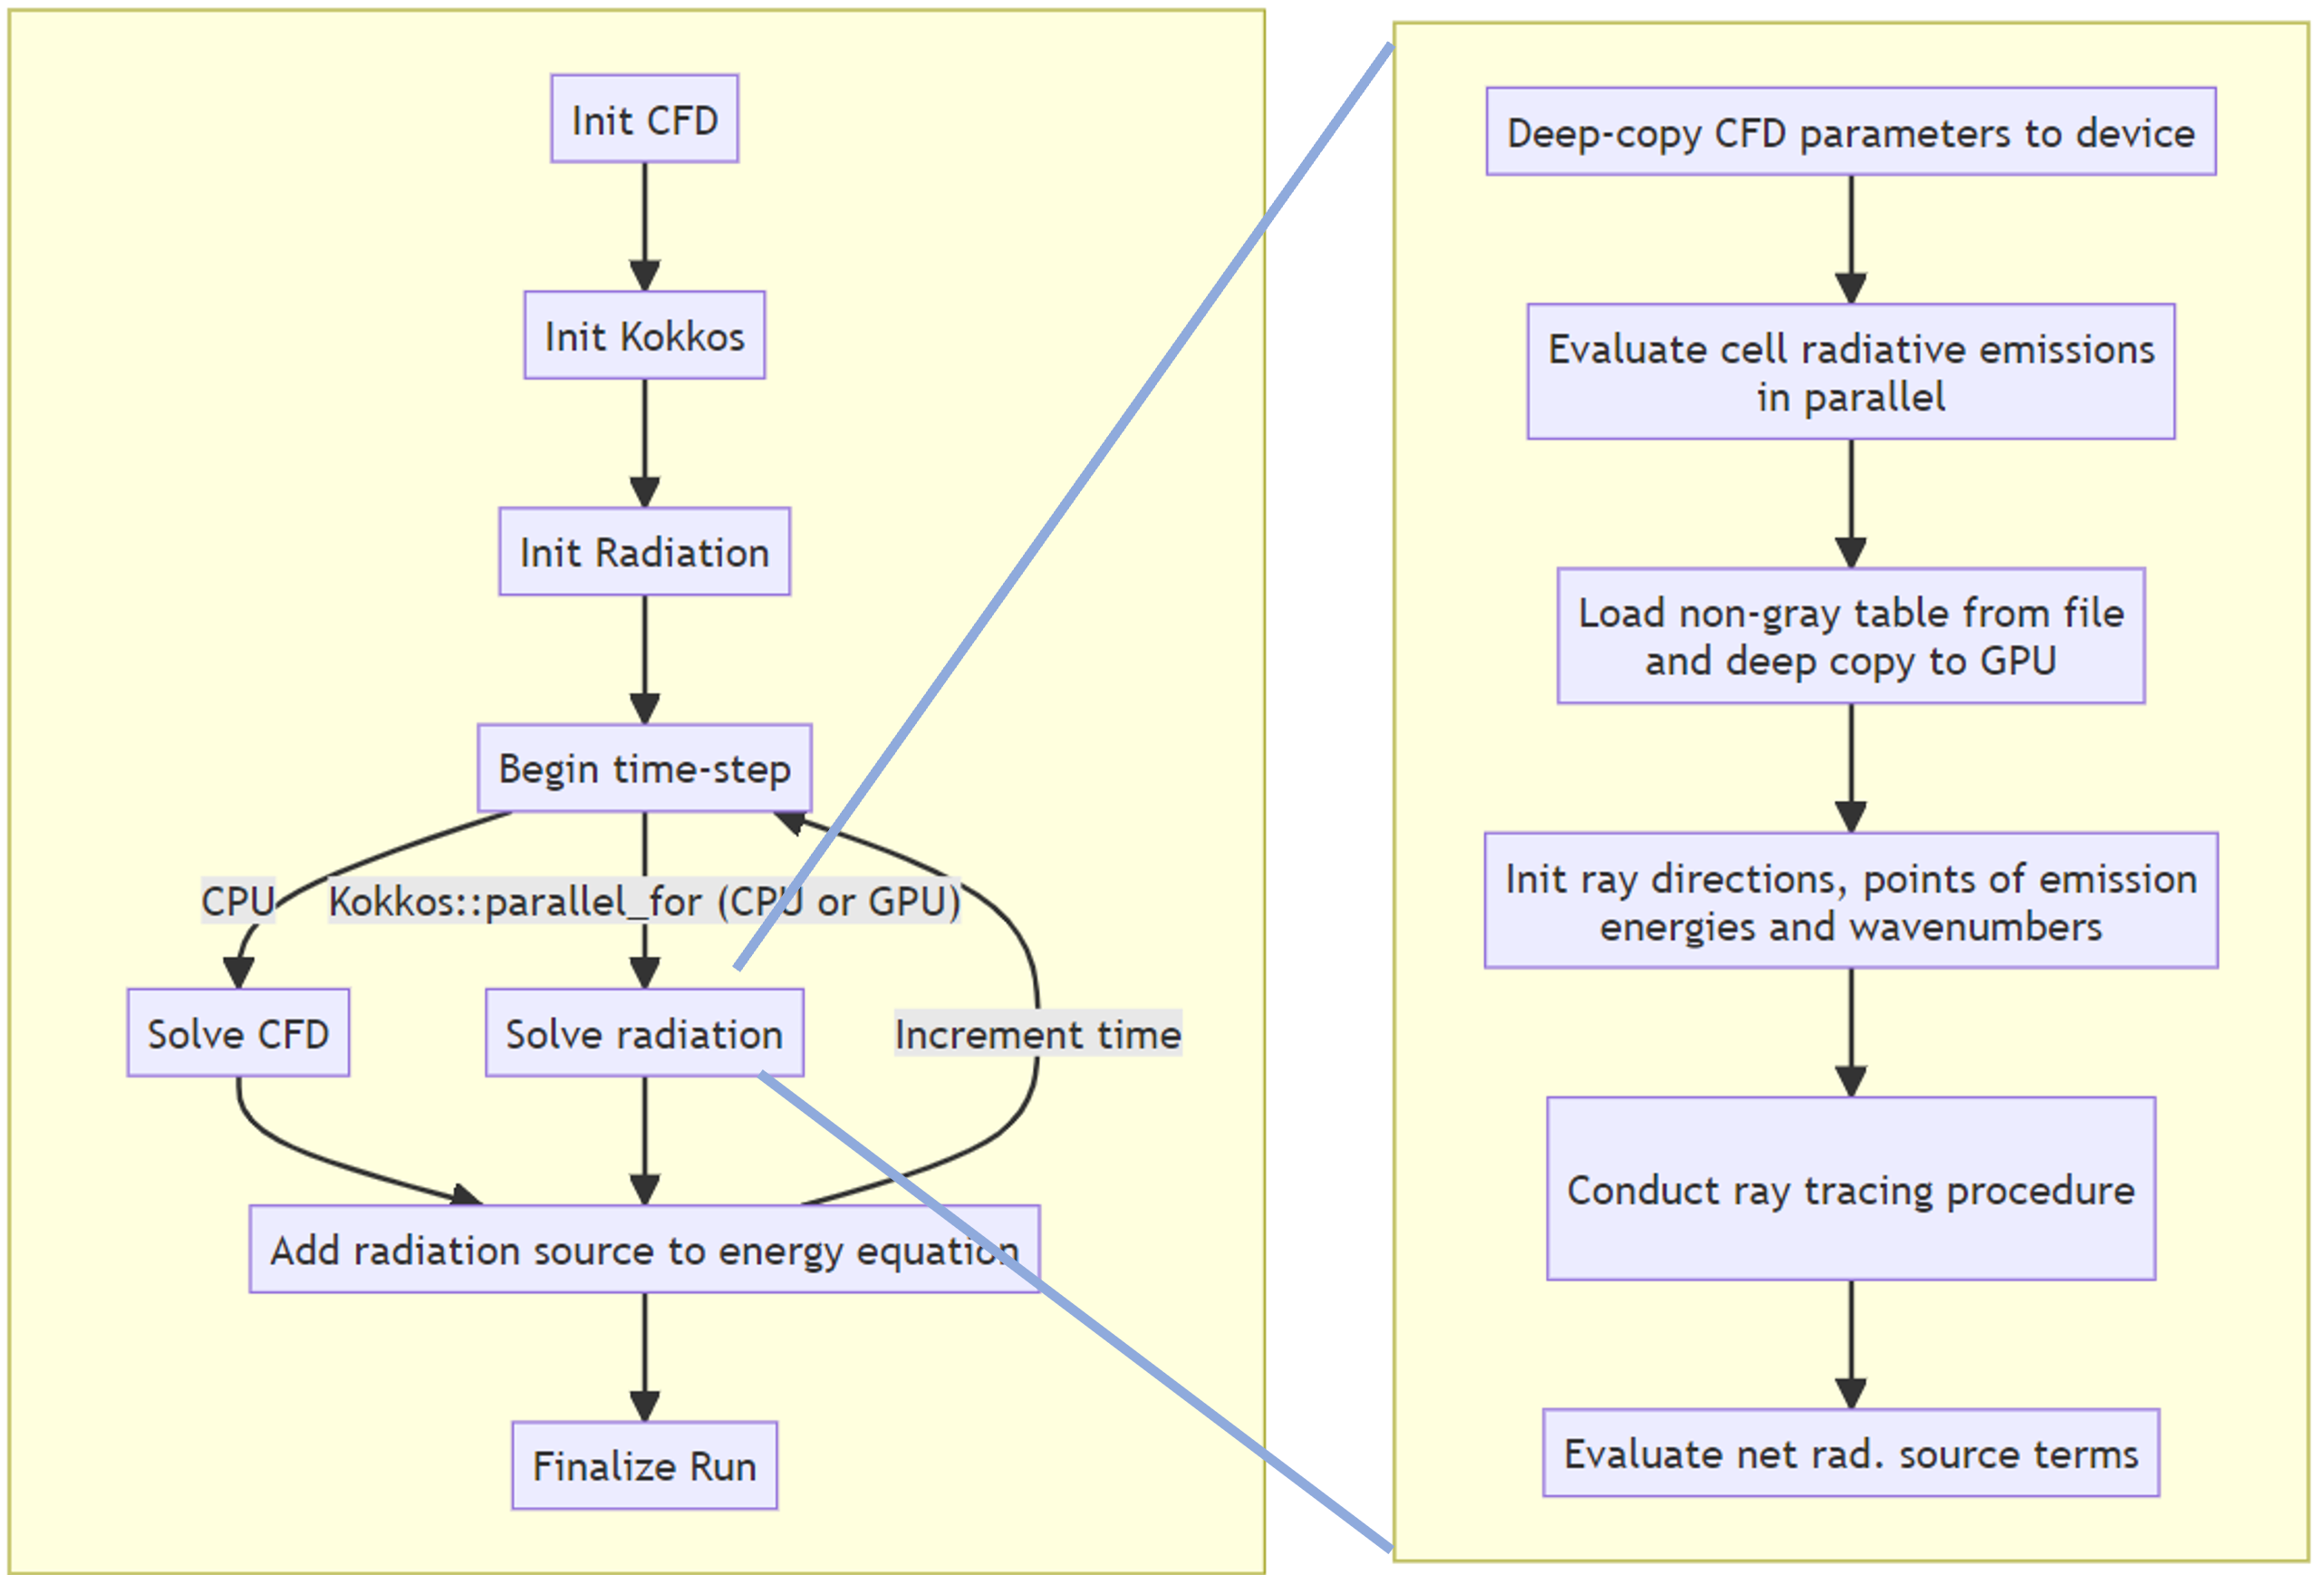
\includegraphics[width=\linewidth]{figures/ch3/joint_flow_chart.png}
  \caption{Streamlines traced from the entrance of the BFS.}
  \label{fig:joint_flow_chart}
\end{figure}


\begin{figure}
  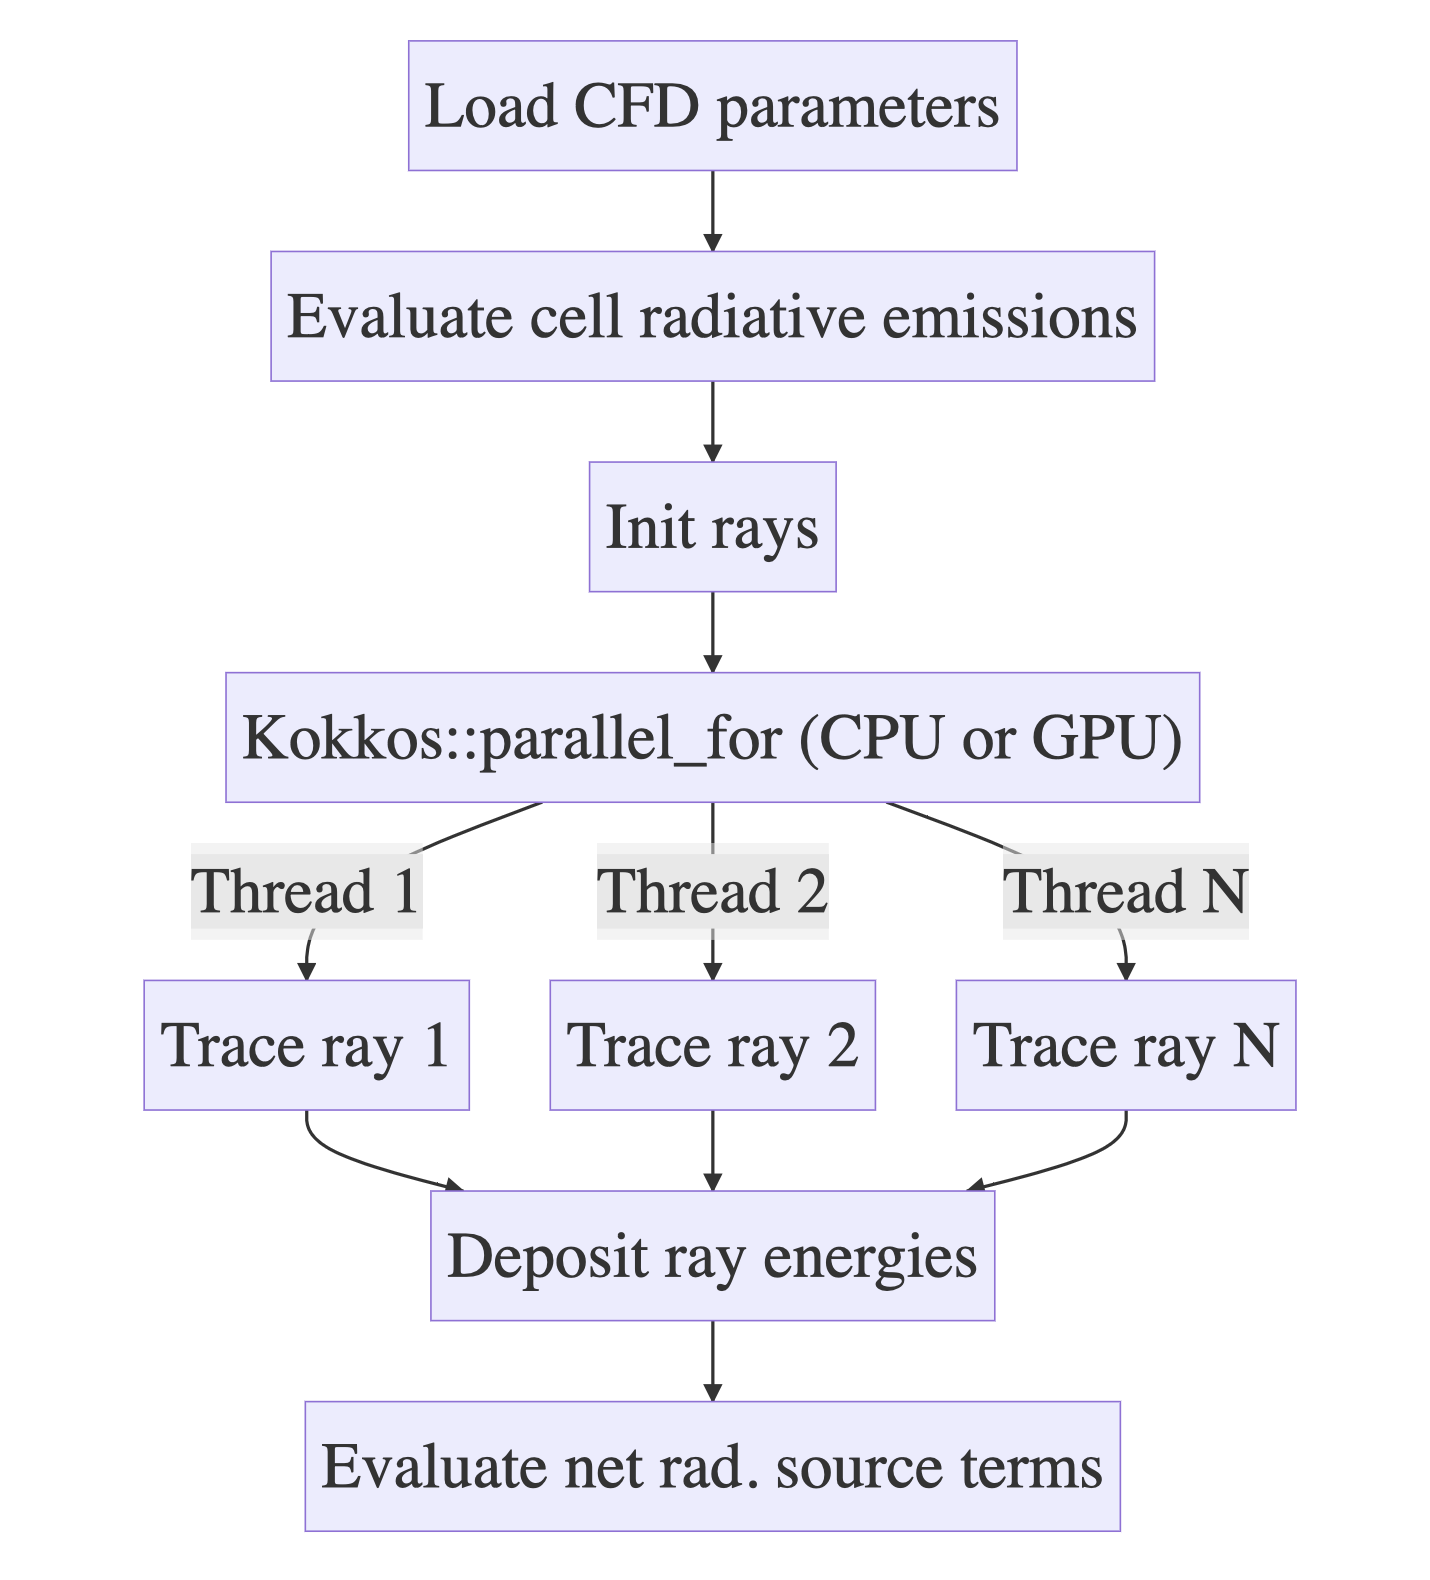
\includegraphics[width=\linewidth]{figures/ch3/radiation_flow_chart.png}
  \caption{BFS temperature contour along the mid-plane. }
  \label{fig:MCRT_flow_chart}
\end{figure}


\subsection{Description of the code}
Following the implementations discussed by \citet{Silvestri2019ASimulation} and \citet{Humphrey2015ATracing}, we implement an MCRT model on GPUs. 
This code connects to the OpenFOAM open-sourced CFD platform \cite{Weller1998ATechniques}, can run on distributed memory systems for scalable computation, and optionally uses a BVH to accelerate the geometric search process of the ray-box and ray-node intersections.
Our code consists of more than 2,000 lines of C++ code, and relies on the Kokkos programming model for a performance-portable parallelization framework \cite{Trott2021KokkosEra}, and the ArborX geometric search library for optimal BVH tree management and traversal functions (which itself relies on Kokkos) \cite{Lebrun-Grandie2019ArborX:Library}.


\subsubsection{OpenFOAM}
With OpenFOAM\footnote{https://github.com/OpenFOAM/OpenFOAM-5.x}, this code can be applied to any CFD solver of interest enabling its use in applications from aeronautical combustor engineering to fire suppression and management. OpenFOAM provides an extensive list of supplemental libraries, allowing the user to model RANS, LES, or DNS simulations with multi-phase flow and detailed chemistry. 
Time-accurate simulations can be implemented with MCRT-GPU with or without Adaptive Mesh Refinement (AMR) on polyhedral, unstructured mesh.
Users can adapt their own OpenFOAM solvers to use MCRT-GPU, or use the default examples for reactingFoam and fireFoam. Instructions are available in the public repository (or private?).

\subsubsection{Kokkos}
Kokkos~\footnote{https://github.com/kokkos} is a performance-portable programming model from the Department of Energy \cite{Trott_Kokkos3_2022,TrottKokkosOGPaper2014}. 
Targeted for HPCs, Kokkos provides abstractions over the parallel execution process and memory management in your solver. By programming in Kokkos, the user can neglect many worries about the underlying parallel execution process and instead focus on their code.
Kokkos supports CUDA, HIP, SYCL, HPX, OpenMP and C++ threads as parallel backends, which the user can easily switch between at compile time.
Additionally, the Kokkos ecosystem streamlines the debugging and profiling process \cite{Trott_KokkosEcosystem2021}.

\subsubsection{ArborX}
Following the Bounding Volume Hierarchy (BVH) description from \citet{Karras2012MaximizingTrees}, ArborX~\footnote{https://github.com/arborx/ArborX} provides a parallel implementation for both spatial-search and nearest-neighbor calculations using a BVH \cite{Lebrun-Grandie2019ArborX:Library}.

The ArborX API enables usage of the BVH through a two-step process: construction and traversal. The user can define \textit{primitives}, or underlying objects with labeled bounding-boxes, and ArborX will efficiently construct a balanced BVH for usage with any parallel backend (using Kokkos). Then, the user can define \textit{predicates} which define the operation the traversal process will be conducting (i.e. spatial search criteria) while traversing the tree.
MCRT-GPU enables the user to optionally use the BVH through ArborX to optimize the ray-tracing procedure. The \textit{primitives} are the computational cells in the CFD process (convex polyhedrons), and the \textit{predicates} are the rays traveling through space.

ArborX uses Kokkos as a backend for on-node parallelism, and implements additional MPI functionality to extend the BVH query process across multi-node runs. Distributed memory executions proceed through an upper-tree and lower-tree approach.
Each node contains knowledge of an upper-tree, which defines defines a BVH for each of the nodes in domain-decomposed space. Then, the lower tree represents the BVH for the computational cells that exist from the CFD solver. 
MCRT-GPU applies ray-tracing procedure across the distributed memory system using this method, which provides enhancement over the traditional MPI iteration approach as discussed in section \ref{sec:DistMemAccel}.

\subsubsection{Non-gray model}
MCRT-GPU has been built to enable use with one of three nongray models: line-by-line, gray modeling with a user-defined absorption coefficient, or gray modeling with planck-mean absorption coefficients. Non-gray databases can be derived from HITEMP or other means with CO$_2$, H$_2$O, and CO spectral lines \cite{Rothman2010HITEMPDatabase} following the approach from .


\subsubsection{User functionality}
MCRT-GPU is meant to be an adaptable radiation model that can be quickly linked to the user's OpenFOAM solver for fast and accurate radiation modeling during their time-accurate CFD simulation.

While the BVH may enable faster computation, in absence of proper development there exist both a version with and without its use.
The version without applies the traditional Monte-Carlo algorithms with Kokkos acceleration. This enables fast GPU-acceleration, with line-by-line non-gray modeling, ray-reflections, and distributed-memory calculation.

Users can access the code through a public repository on github \footnote{https://github.com/nick-jt/MCRT-GPU}.

\subsection{Distributed Memory Acceleration}\label{sec:DistMemAccel}